\documentclass{beamer}
\usepackage[italian]{babel}
\usepackage{graphicx}
\usepackage{listings}
\usepackage{xcolor}
\usepackage{graphicx}
\usepackage{subcaption}

\usepackage{eso-pic} % Pacchetto per inserire elementi grafici

\usetheme{Madrid}
\usecolortheme{whale}

\title{Gestione Progetti: Un'Applicazione Robusta e Testata}
\author{Elena Zerbin}
\date{\today}

% Definizione di un linguaggio personalizzato per YAML
\lstdefinelanguage{yaml}{
  basicstyle=\ttfamily\small,
  morekeywords={true,false,null,y,n},
  sensitive=false,
  morecomment=[l]{\#},
  morestring=[b]',
  morestring=[b]",
  commentstyle=\color{gray}\ttfamily,
  keywordstyle=\color{blue}\ttfamily,
  stringstyle=\color{purple}\ttfamily,
  showstringspaces=false,
  breaklines=true
}

% Definizione di un linguaggio personalizzato per YAML
\lstdefinelanguage{Dockerfile}{
  basicstyle=\ttfamily\small,
  morekeywords={true,false,null,y,n},
  sensitive=false,
  morecomment=[l]{\#},
  morestring=[b]',
  morestring=[b]",
  commentstyle=\color{gray}\ttfamily,
  keywordstyle=\color{blue}\ttfamily,
  stringstyle=\color{purple}\ttfamily,
  showstringspaces=false,
  breaklines=true
}

\begin{document}

\frame{\titlepage}

\begin{frame}
\frametitle{1. Introduzione}
Benvenuti alla presentazione del nostro sistema di Gestione Progetti.
\end{frame}

\begin{frame}
\frametitle{2. Architettura del Database}
\framesubtitle{Diagramma ER}
\begin{figure}
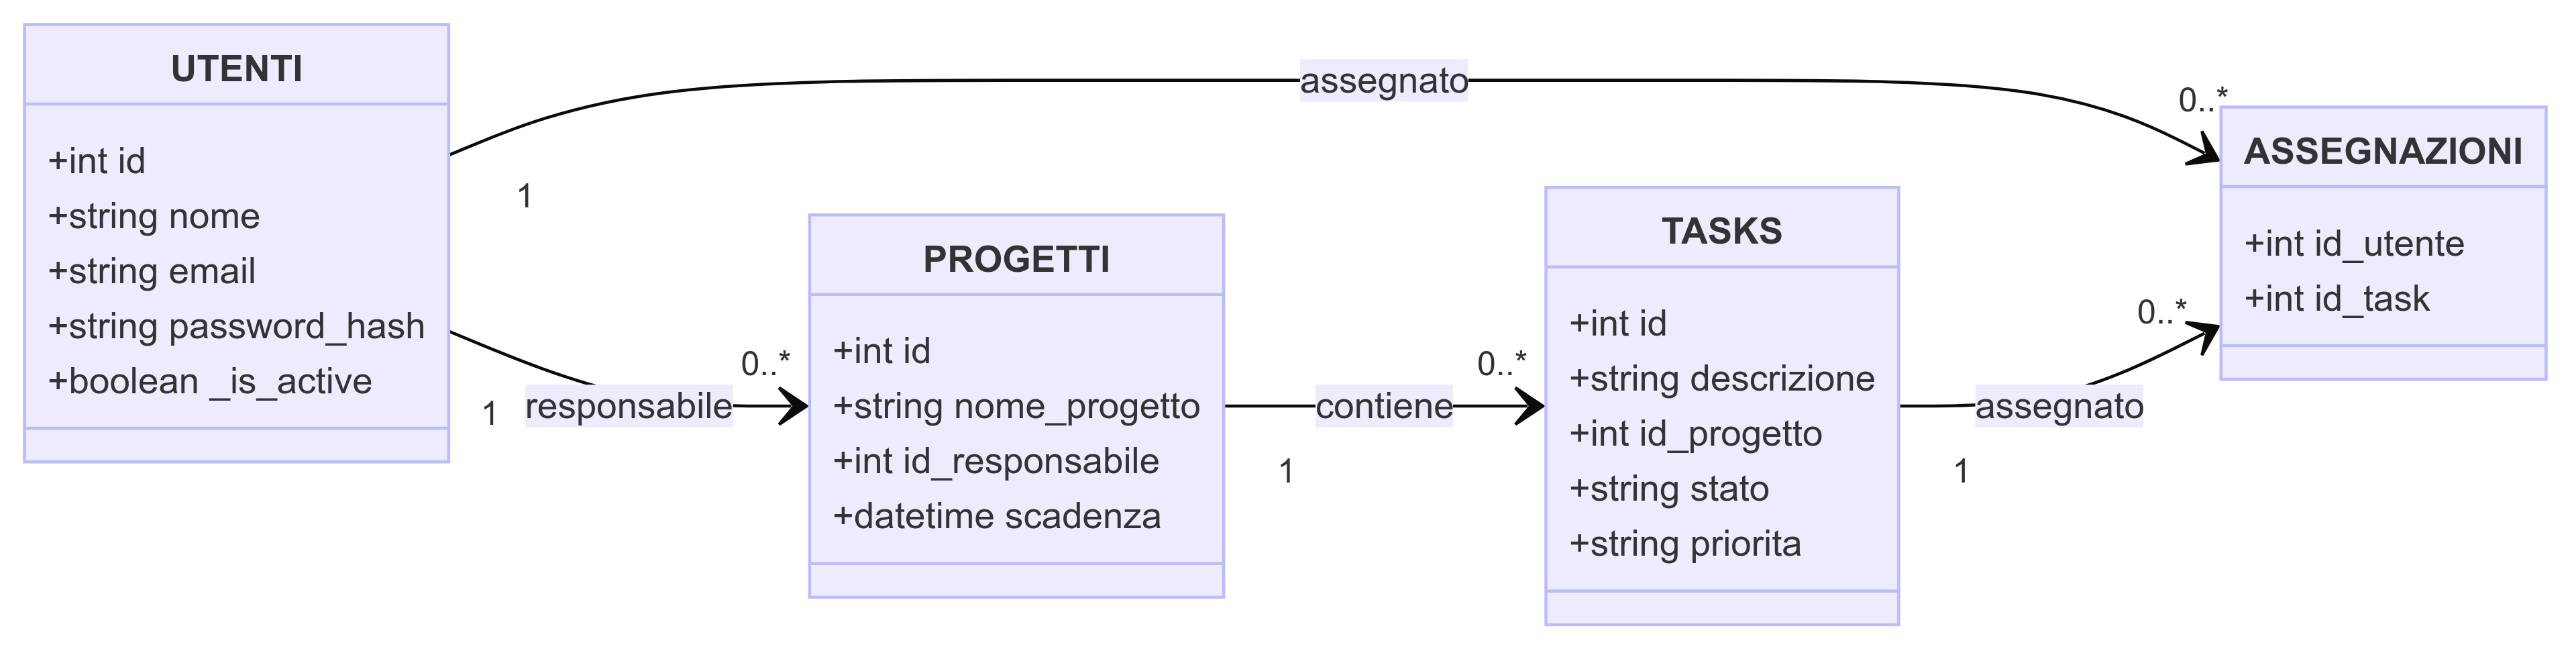
\includegraphics[width=\textwidth]{diagramma_ER.png}
\caption{Diagramma ER del nostro database}
\end{figure}
\end{frame}

\begin{frame}
\frametitle{3. Funzionalità Principali}
\begin{enumerate}
\item Registrazione e autenticazione utenti
\item Creazione e gestione di progetti
\item Aggiunta e gestione di task
\item Assegnazione di task agli utenti
\item Monitoraggio dello stato e della priorità
\item Gestione delle scadenze
\end{enumerate}
\end{frame}

\begin{frame}
\frametitle{4. Tecnologie Utilizzate}
\begin{itemize}
\item Backend: Python con Flask
\item Database: MySQL
\item Testing: pytest, Hypothesis
\end{itemize}
\end{frame}

\begin{frame}[fragile]
\frametitle{5. Test e Qualità del Codice}
\framesubtitle{5.1 Test Unitari con Property-Based Testing}
Utilizzo Hypothesis per il property-based testing, che ci permette di generare automaticamente una vasta gamma di input di test.

\begin{figure}
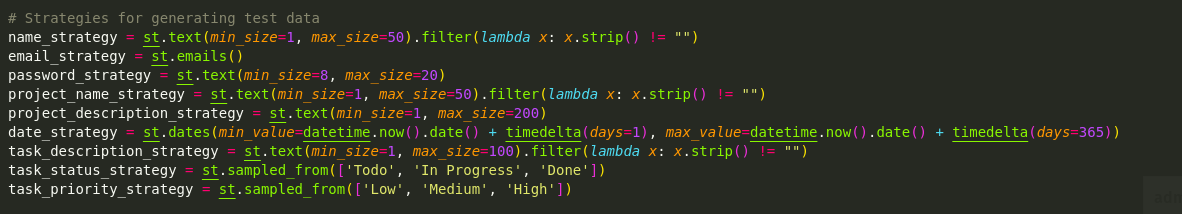
\includegraphics[width=\textwidth]{test_data.png}
\caption{Strategie per la generazione di dati di prova}
\end{figure}

Questi test ci permettono di:
\begin{itemize}
\item Verificare la robustezza delle nostre funzioni con input diversificati
\item Scoprire edge case che potrebbero sfuggire ai test tradizionali
\item Assicurare che le nostre funzioni rispettino determinate proprietà invarianti
\end{itemize}
\end{frame}

\begin{frame}[fragile]
\frametitle{5. Test e Qualità del Codice}
\framesubtitle{5.2 Test di Integrazione Completi}
Questi test coprono l'intero flusso dell'applicazione, dalla registrazione dell'utente alla creazione e gestione di progetti e task.

\begin{itemize}
    \item Tutte le funzionalità del test parziale
    \item Test di Scenari di Errore Specifici
    \item Test di Funzionalità Aggiuntive (Modifica Progetti e Tasks)
    \item Test per API o Endpoints Aggiuntivi
    \item Test di Eliminazione di Progetti e Tasks Non Esistenti
\end{itemize}

\textbf{Note:}
\begin{itemize}
    \item Copertura più completa delle funzionalità e degli scenari di errore.
    \item Include test specifici per API e gestione di errori.
\end{itemize}

\end{frame}

\begin{frame}[fragile]
\frametitle{5. Test e Qualità del Codice}
\framesubtitle{5.3 Test di Integrazione Parziali}
Questi test si concentrano su specifiche funzionalità o scenari, come:

\begin{itemize}
    \item \textbf{Registrazione, Login e Logout:}
    \begin{itemize}
        \item Registrazione di un nuovo utente.
        \item Login con le credenziali dell'utente registrato.
        \item Logout dell'utente.
    \end{itemize}
    
    \item \textbf{CRUD Progetto:}
    \begin{itemize}
        \item Creazione di un progetto con validazione del nome del progetto.
        \item Creazione di un progetto valido.
        \item Verifica della creazione del progetto nel database.
        \item Eliminazione di un progetto.
        \item Verifica dell'eliminazione del progetto nel database.
    \end{itemize}
\end{itemize}
\end{frame}

\begin{frame}[fragile]
\frametitle{5. Test e Qualità del Codice}
\framesubtitle{5.3 Test di Integrazione Parziali (continua)}
\begin{itemize}
    \item \textbf{CRUD Task:}
    \begin{itemize}
        \item Creazione di un progetto per associarlo ai task.
        \item Creazione di un task valido associato al progetto.
        \item Verifica della creazione del task nel database.
        \item Eliminazione di un task.
        \item Verifica dell'eliminazione del task nel database.
    \end{itemize}
    
    \item \textbf{Accesso Non Autorizzato:}
    \begin{itemize}
        \item Tentativo di accesso alla dashboard senza autenticazione.
        \item Tentativo di aggiungere un progetto senza autenticazione.
        \item Tentativo di aggiungere un task senza autenticazione.
    \end{itemize}
\end{itemize}
\end{frame}

\begin{frame}
\frametitle{5. Test e Qualità del Codice}
\framesubtitle{Risultati dei Test}
\begin{figure}[h!]
    \centering
    \begin{subfigure}[b]{0.45\textwidth}
        \centering
        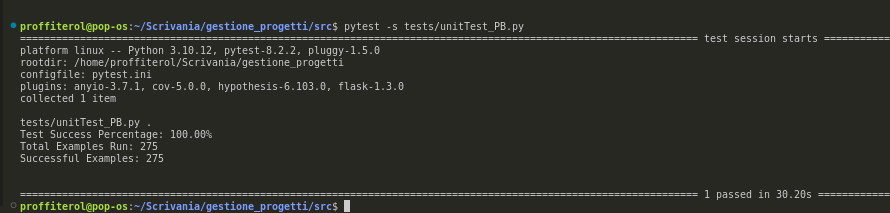
\includegraphics[width=\textwidth]{test_PB.png}
        \caption{Property based Testing}

    \end{subfigure}
    \hfill
    \begin{subfigure}[b]{0.45\textwidth}
        \centering
        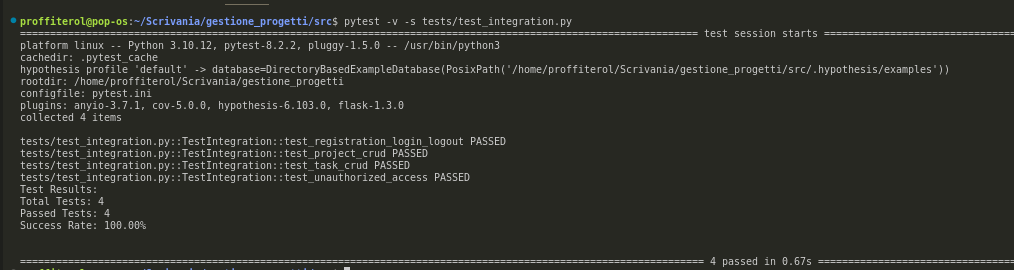
\includegraphics[width=\textwidth]{test_integration.png}
        \caption{test integration parziale}
    \end{subfigure}
      \hfill
    \begin{subfigure}[b]{0.45\textwidth}
        \centering
        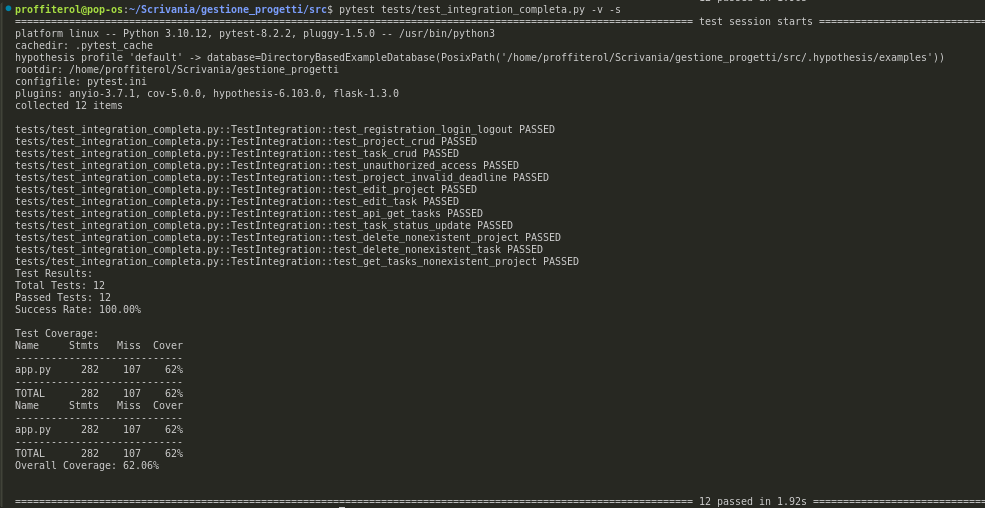
\includegraphics[width=\textwidth]{test_integration_completa.png}
        \caption{test integration completa}
    \end{subfigure}
\end{figure}
\end{frame}

\begin{frame}[fragile]
\frametitle{5. Test e Qualità del Codice}
\framesubtitle{5.4 Misura della Copertura dei Test}
Utilizziamo il modulo coverage di Python per misurare la copertura dei nostri test.

Processo:
\begin{itemize}
\item Esecuzione dei test con copertura attivata
\item Generazione di un report dettagliato
\item Analisi delle aree del codice non coperte dai test
\end{itemize}

\begin{lstlisting}[basicstyle=\tiny]
Test Results:
Total Tests: 12
Passed Tests: 12
Success Rate: 100.00%

Test Coverage:
Name                 Stmts   Miss  Cover
----------------------------------------
app                    282     107    62%
----------------------------------------
TOTAL                  282     107    62%
----------------------------------------
Overall Coverage 62.06%
\end{lstlisting}
\end{frame}

\begin{frame}[fragile]
\frametitle{6. Continuous Integration e Continuous Delivery}
\framesubtitle{Pipeline CI/CD}

\begin{itemize}
\item La pipeline CI/CD automatizza il processo di build, test e deploy del codice.
\item Utilizziamo GitHub Actions per implementare la pipeline.
\end{itemize}

\textbf{Configurazione della Pipeline:}

\begin{figure}[h!]
    \centering
    \begin{subfigure}[b]{0.45\textwidth}
        \centering
        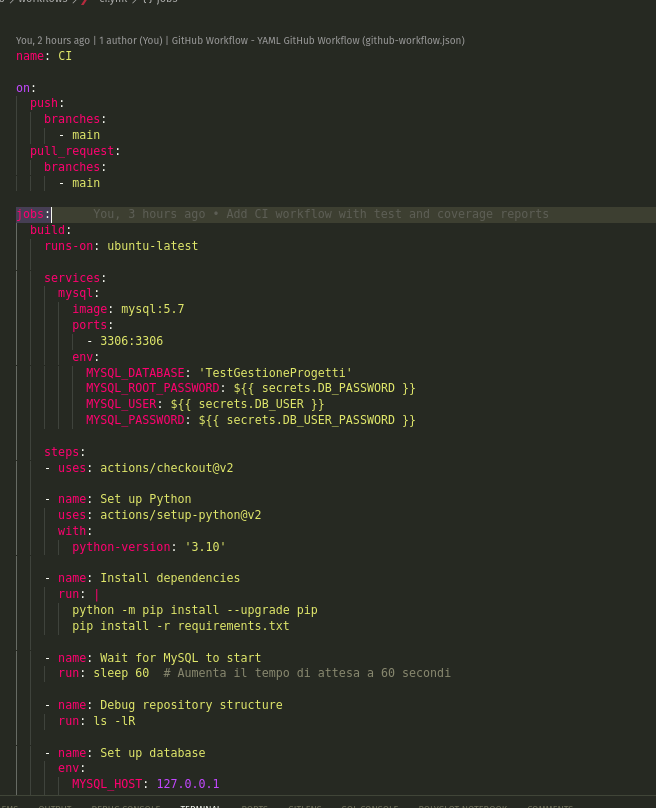
\includegraphics[width=3cm]{img1.png}
        \caption{Config. della Pipeline parte 1}
    \end{subfigure}
    \hfill
    \begin{subfigure}[b]{0.45\textwidth}
        \centering
        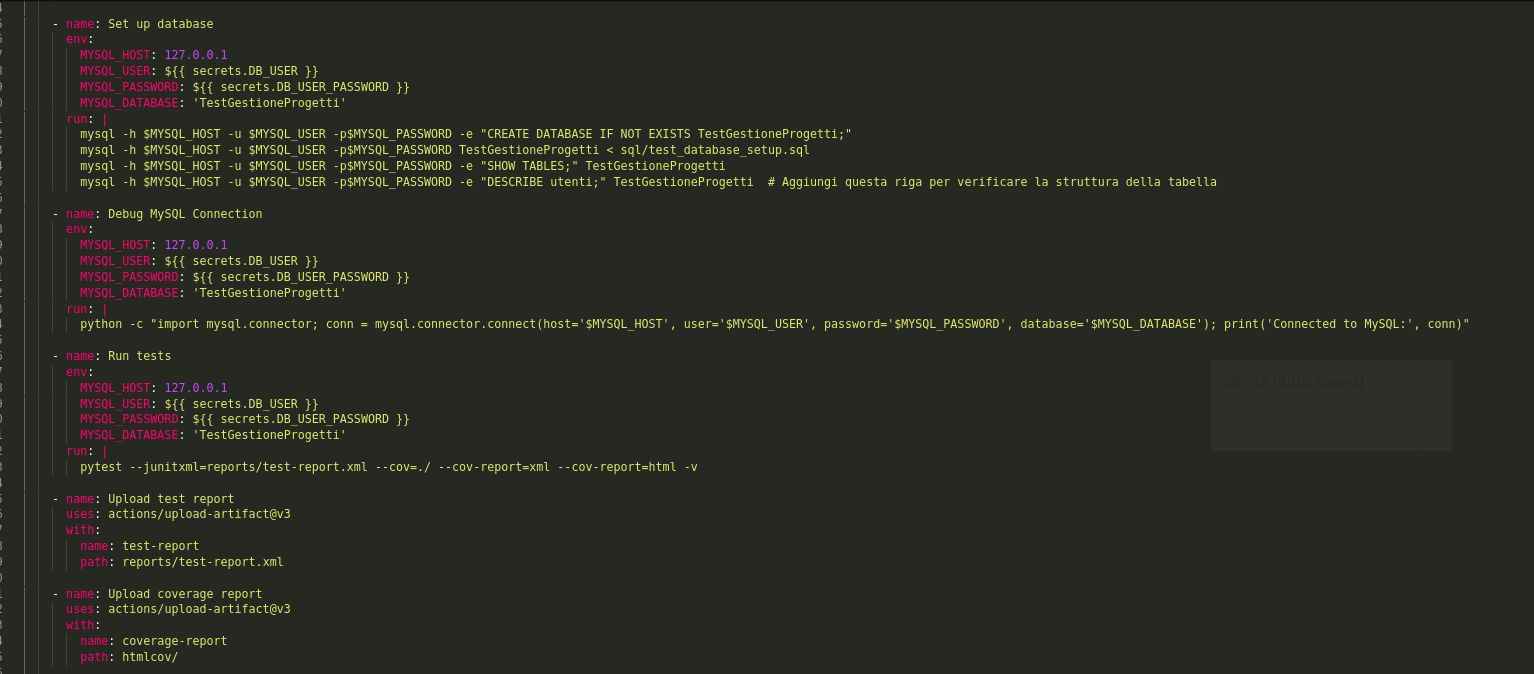
\includegraphics[width=\textwidth]{img2.png}
        \caption{Config. della Pipeline parte 2}

    \end{subfigure}
\end{figure}
\end{frame}

\begin{frame}[fragile]
\frametitle{7. Deployment in Container}
\framesubtitle{Pipeline CI/CD con Docker}

\begin{itemize}
\item La pipeline CI/CD automatizza il processo di build, test e deploy del codice.
\item Utilizziamo GitHub Actions per implementare la pipeline e Docker per il deployment.
\end{itemize}

\textbf{Configurazione della Pipeline:}
\begin{lstlisting}[language=yaml, basicstyle=\tiny]
    - name: Log in to Docker Hub
      uses: docker/login-action@v2
      with:
        username: ${{ secrets.DOCKER_USERNAME }}
        password: ${{ secrets.DOCKER_PASSWORD }}

    - name: Build and push Docker image
      run: |
        IMAGE_NAME=${{ secrets.DOCKER_USERNAME }}/gestione_progetti
        IMAGE_TAG=${GITHUB_SHA::7}
        docker build -t $IMAGE_NAME:$IMAGE_TAG .
        docker push $IMAGE_NAME:$IMAGE_TAG
        docker tag $IMAGE_NAME:$IMAGE_TAG $IMAGE_NAME:latest
        docker push $IMAGE_NAME:latest
\end{lstlisting}
\end{frame}

\begin{frame}[fragile]
\frametitle{7. Deployment in Container}
\framesubtitle{Dockerfile}

\begin{itemize}
\item Utilizziamo Docker per creare un'immagine containerizzata dell'applicazione.
\item Ecco il Dockerfile usato per costruire l'immagine.
\end{itemize}

\textbf{Dockerfile:}
\begin{lstlisting}[language=Dockerfile, basicstyle=\tiny]
# Usa un'immagine base Python
FROM python:3.10-slim

# Imposta la directory di lavoro nel container
WORKDIR /app

# Copia i file requirements.txt e installa le dipendenze
COPY requirements.txt requirements.txt
RUN pip install --no-cache-dir -r requirements.txt

# Copia il resto del codice dell'applicazione nel container
COPY . .

# Espone la porta su cui gira l'applicazione
EXPOSE 5000

# Comando per eseguire l'applicazione
CMD ["python", "src/app.py"]
\end{lstlisting}
\end{frame}


\begin{frame}
\frametitle{Grazie!}
\centering
Grazie per l'attenzione
\end{frame}

\end{document}
